\section{Design}

% This is where the logical / abstract contribution of the project is presented.

% Notice that, when describing a software project, three dimensions need to be taken into account: structure, behaviour, and interaction.

% Always remember to report \textbf{why} a particular design has been chosen.
% Reporting wrong design choices which has been evalued during the design phase is welcome too.

In questa sezione si analizza il sistema AMW da punto di vista di \textit{struttura}, \textit{comportamento} ed \textit{interazione}.
Si discuterà inizialmente la struttura di massima del sistema e le entità rappresentate. Successivamente, si analizzerà il loro comportamento. Infine verranno presentate le modalità di interazione.

\subsection{Struttura}

% Which entities need to by modelled to solve the problem?
% %
% (UML Class diagram)
% How should entities be modularised?
% %
% (UML Component / Package / Deployment Diagrams)

Il sistema AMW è un software distribuito basato sull'astrazione degli agenti, che definiscono la struttura e le comunicazioni di ogni singola entità del magazzino. Questi sono dunque molteplici e la loro interazione permette al behaviour complessivo del magazzino di emergere.\\
Nello specifico, gli agenti che concorrono al corretto funzionamento del sistema sono:
\begin{itemize}
    \item Admin
    \item User
    \item Collection Point Manager
    \item Command Manager
    \item Order Manager
    \item Robot Picker
    \item Warehouse Mapper
\end{itemize}
Ogni agente svolge un preciso compito e interagisce con uno o più agenti differenti. Ciò permette al comportamento complessivo del sistema di emergere dall'interazione delle sue sotto componenti (TODO).\\
All'interno del sistema si è testata la presenza di una singola istanza di ogni agente (ad eccezion fatta per gli agenti client e robotici TODO). Ciò non impedisce tuttavia di aggiungerne di nuovi, in quando la scoperta di questi viene effettuata runtime tramite un servizio di pagine gialle, che quindi permette una loro aggiunta in maniera flessibile.\\
L'unico punto contrario alla dichiarazione precedente potrebbe riguardare il Collection Point Manager, che gestisce infatti l'allocazione di componenti fisiche e necessiterebbe quindi di una ridondanza effettuata in maniera oculata.
% TODO all’interno del sistema sono presenti una sola istanza di ogni agente sopra elencato, ad eccezione del User. Per questo agente, il numero di istanze corrisponde al numero di clienti al lavoro e può variare durante l’esecuzione.
\parag
Di seguito verrà fornita una descrizione della struttura degli agenti. A tal scopo risulta però necessario fornire una rappresentazione propedeutica dell'ambiente, definita tramite l'utilizzo di un'ontologia.

\subsubsection{Ontologia del sistema}
Un ontologia rappresenta un sistema in quanto tale, le categorie fondamentali che lo compongono e le relazioni fra esse. Questa è una componente importante per la rappresentazione della conoscenza ed è stata utilizzata nel sistema per descrivere e definire l'ambiente del magazzino e le operazioni ad esso relative.\\
Nello specifico, è stata definita un'ontologia relativa agli oggetti fisici o informativi ed alle loro relazioni (vedasi Figura \ref{fig:ontology_abstractions}); ed una ontologia relativa alle operazioni su di essi effettuabili (vedasi Figure \ref{fig:ontology_operations-1} e \ref{fig:ontology_operations-2}).
%
\parag
Le entità fisiche rappresentate nel sistema magazzino sono gli \textit{item}, ovvero gli oggetti ordinabili in esso conservati. Questi sono rappresentati da un \textit{id} univoco e mantenuti, in differenti \textit{quantity}, in scaffalature identificabili da una coppia \textit{rack-value}.\\
Per quanto riguarda le entità puramente informative, si possono riscontrare i \textit{command} e le informazioni relative agli \textit{user} del sistema. Le prime sono relative al \textit{repository} di conoscenza procedurale a cui gli agenti possono attingere; le seconde sono relative alle informazioni, quali l'indirizzo di spedizione, utilizzate durante la sottomissione di un \textit{order}. Quest'ultimo contiene le informazioni relative all'ordine dell'utente, insieme al \textit{collection point} (i.e., il punto di raggruppamento dei prodotti) e allo \textit{status}. Si sottolinea infine come l'astrazione dell'order sia utilizzata dal solo agente \textit{order-manager}, in quanto gli altri agenti accedono solo alle informazioni ad esso correlate.
\begin{figure}[ht]
    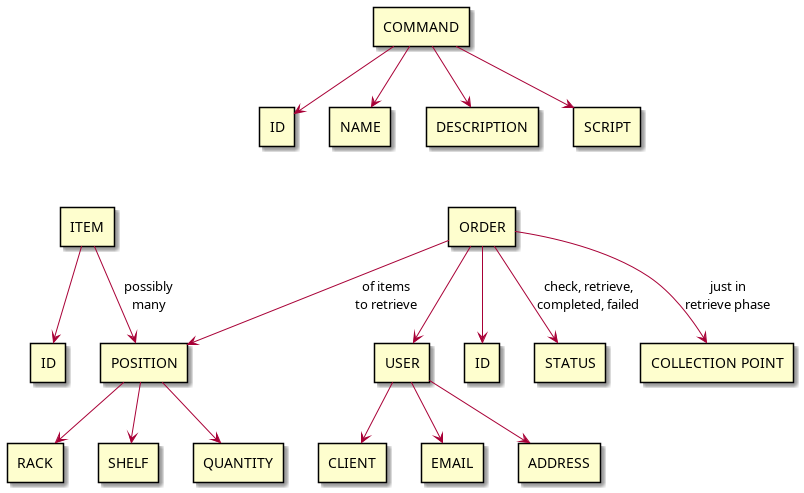
\includegraphics[width=\textwidth]{section/design/figure/ontology/ontology-abstractions.png}
    \caption{Schema relazionale delle entità fisiche e concettuali rappresentate nel sistema.}
    \label{fig:ontology_abstractions}
\end{figure}
%
\parag
L'ontologia rappresentante le operazioni definisce invece le azioni che possono coinvolgere determinate astrazioni del sistema e le informazioni per la loro esecuzione. Un banale esempio di ciò è l'operazione di piazzamento di un ordine, la quale necessita di mettere in relazione informazioni associate all'acquirente e gli oggetti richiesti da questo.
\begin{figure}[!ht]\centering
    \includegraphics[width=.7\textwidth]{section/design/figure/ontology/ontology-operations-1.png}% TODO
    \caption{Parziale rappresentazione schematica delle operazioni disponibili nel sistema e delle loro relazioni con le astrazioni precedentemente definite. Questa parte mostra le operazioni relative ad ordini e prodotti.}
    \label{fig:ontology_operations-1}
\end{figure}
\begin{figure}[!ht]\centering
    \includegraphics[width=\textwidth]{section/design/figure/ontology/ontology-operations-2.png}% TODO
    \caption{Parziale rappresentazione schematica delle operazioni disponibili nel sistema e delle loro relazioni con le astrazioni precedentemente definite. Questa parte mostra le operazioni relative a comandi e punti di raccolta.}
    \label{fig:ontology_operations-2}
\end{figure}%TODO commenti frecce

\subsubsection{Admin}
L'agente admin \`e colui che si occupa di permettere l'interazione dell'amministratore col sistema. Condividendo alcuni tratti con l'agente user, si \'e deciso di raccogliere le caratteristiche comuni di queste due entit\'a tramite la definizione di un agente astratto dedito alla comunicazione col sistema (in esso, \'e denominato \textit{Communicator}; vedasi Figura \ref{fig:class_diagram_admin_agent}).\\
Le funzionalit\'a principali dell'agente admin sono relative alla gestione del magazzino e all'esecuzione di comandi nel sistema. Ricercando una separazione dei privilegi, questo non \'e in grado di effettuare ordini.
\begin{figure}[ht]
    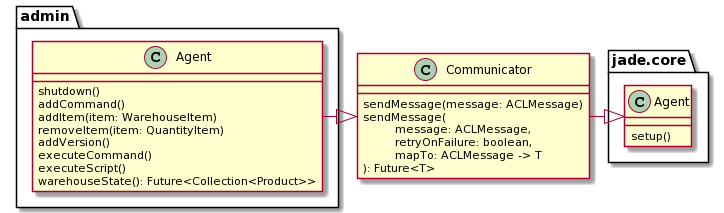
\includegraphics[width=\textwidth]{section/design/figure/admin/class_diagram.png}
    \caption{Diagramma delle classi dell'agente utilizzato per la comunicazione admin-sistema.}
    \label{fig:class_diagram_admin_agent}
\end{figure}

\subsubsection{User}
L'agente user si occupa di permettere l'interazione degli utenti/acquirenti col sistema. Come gi\'a accennato, condivide alcuni tratti con l'agente admin: questi sono accomunati dall'estensione dell'agente \textit{Communicator} (vedasi Figura \ref{fig:class_diagram_user_agent}).\\
Le funzionalit\'a principali dell'agente user consistono nella possibilit\'a di effettuare ordini e vederne lo stato (TODO). Non \'e invece dotato della capacit\'a di 'modificare' direttamente il magazzino, in quanto si tratta di una capacit\'a disponibile al solo amministratore.
\begin{figure}[ht]
    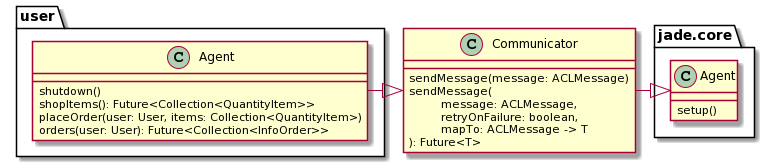
\includegraphics[width=\textwidth]{section/design/figure/user/class_diagram.png}
    \caption{Diagramma delle classi dell'agente utilizzato per la comunicazione user/client-sistema.}
    \label{fig:class_diagram_user_agent}
\end{figure}

\subsubsection{Collection Point Manager}
\subsubsection{Command Manager}
\subsubsection{Order Manager}
\subsubsection{Robot Picker}
\subsubsection{Warehouse Mapper}

\subsection{Comportamento}

% How should each entity behave?
% %
% (UML State diagram or Activity Diagram)

Come già anticipato, gli agenti del sistema sono sviluppati tramite le tecnologie JADE e Jason. A causa di ciò, i modelli logici delle due tipologie di agenti differiscono, passando da un modello a \textit{behaviour} ad uno \textit{BDI}. Nello specifico, gli agenti sviluppati in JADE ed utilizzanti un modello a behaviour sono quelli relativi al client di interazione col sistema: Admin e User; gli altri agenti sono invece basati sul modello BDI.\\
Di seguito verranno descritti i behaviour e la logica di ogni agente del sistema. Inoltre, verr\'a descritto il comportamento dell'agente 'parziale' \textit{Communicator}, il quale funge da struttura base per gli agenti del lato client.

\subsubsection{Communicator}
Quest'entità parziale permette una gestione delle possibili failure della rete. In pratica, questa si occupa del reinvio dei messaggi in caso non si riceva risposta.\\
L'alternaza dei behaviours \'e visibile nella Figura \ref{fig:communicator_state_diagrams} e rappresenta i comportamenti necessari alla risoluzione dell'errore.\\
Si evidenzia inoltre come, in alternativa a questa forma `\textit{reliable}' di comunicazione, sia sempre possibile utilizzarne una `\textit{unreliable}' senza il reinvio dei messaggi.
\begin{figure}[ht]
    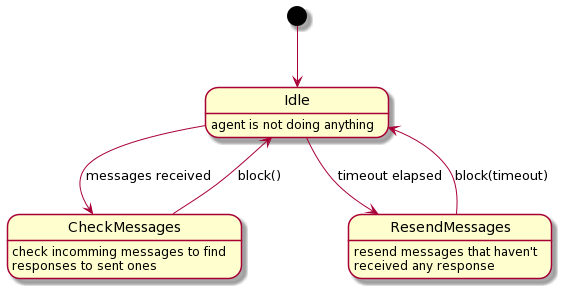
\includegraphics[width=\textwidth]{section/design/figure/agent/communicator_states.png}
    \caption{Diagramma degli stati del \textit{Communicator.} Gli stati diversi da \textit{idle} sono rappresentanti di behaviours dell'agente.}
    \label{fig:communicator_state_diagrams}
\end{figure}

\subsubsection{Admin}
% non ha particolari behaviour aggiuntivi rispetto al communicator in quanto fa solo da interfaccia al client
L'agente admin non ha particolari behaviour aggiuntivi rispetto a quelli di controllo forniti dall'agente \textit{Communicator}. Lo scopo di quest'entit\'a \'e infatti la traduzione dei messaggi dal formato basato su classi/oggetti utilizzato dal client a quello basato su \textit{terms}, \textit{literals}, etc. utilizzato dagli agenti del magazzino. Suo compito \'e infine anche la traduzione delle possibili risposte a questi messaggi.\\% TODO magari fare che il 'de-marshalling' sia un oneshot-behaviour e scriverlo qui.
Per chiarezza, intendiamo sottolineare come il suo compito sia la traduzione dei messaggi e delle risposte relativi alle sole funzionalit\'a disponibili all'admin. Quest'agente non risulta dunque in grado di comprendere le azioni e le entit\'a dell'ontologia utilizzate dal solo utente user.

\subsubsection{User}
% non ha particolari behaviour aggiuntivi rispetto al communicator in quanto fa solo da interfaccia al client
Come per l'entit\'a admin, anche l'user non ha particolari comportamenti aggiuntivi. Il suo compito \'e infatti anch'esso riconducibile alla sola traduzione dei messaggi in ingresso ed in uscita.\\
Anche l'agente user assume un atteggiamento agnostico riguardo i formati delle comunicazioni dell'admin. Esso \'e infatti in grado di comprendere e tradurre le sole componenti dell'ontologia ad esso utili, e non \'e quindi pensato per la comprensione dei messaggi relativi all'amministratore. Questa scelta \'e frutto di una scelta di separazione dei privilegi.

\subsubsection{Collection Point Manager}
Il comportamento dell'agente gestore dei punti di raccolta degli ordini \'e relativamente semplice nella sua comprensione e pu\'o essere schematizzato dal diagramma degli stati visibile in Figura \ref{fig:state-diagram-cpm}. Questo mostra chiaramente come l'agente permetta un'assegnazione di un punto di raccolta per uno specifico ordine quando si trovi in uno stato che ne presenti almeno uno non occupato. L'operazione di \textit{free} si occupa invece di liberarne uno riservato ad un ordine gi\'a completato.%TODO puo essere interessante dire come non posssa risolvere problemi di failure di un order manager in quanto il punto potrebbe gia esser stato occupato?
\parag
Relativamente al diagramma a stati, si ritiene infine importante sottolineare come, trattandosi di un agente BDI, questo non implementi un behaviour per ogni stato in maniera esplicita (TODO check) ma, piuttosto, questo schema comportamentale emerga dall'insieme delle `credenze', `desideri' e `intenzioni' dell'agente stesso.
\begin{figure}
    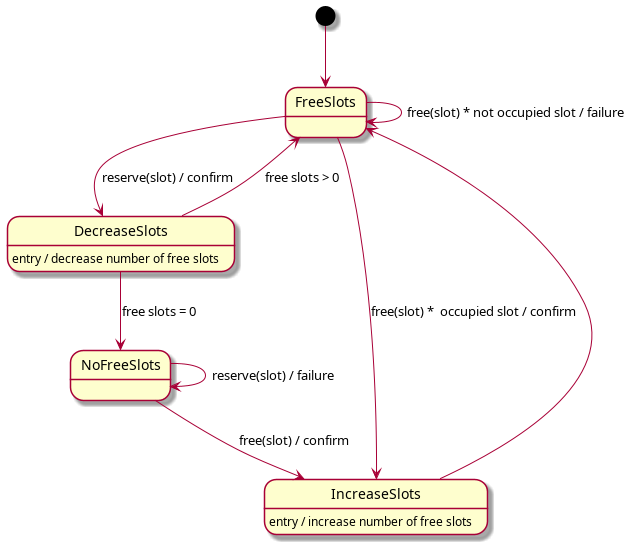
\includegraphics[width=\textwidth]{section/design/figure/collection_point_manager/state_diagram.png}
    \caption{Diagramma a stati schematizzante il comportamento di massima dell'agente \textit{Collection Point Manager}.}
    \label{fig:state-diagram-cpm}
\end{figure}

\subsubsection{Command Manager}
Il comportamento dell'entit\'a del sistema relativa alla gestione del repository di conoscenza e, quindi, dei comandi \'e forse quello meno complesso del sistema. Questo agente si limita infatti a ricevere le richieste e a fornire le risposte. Le possibili richieste a cui deve far fronte riguardano il salvataggio di nuovi comandi (per la gestione del quale deve semplicemente verificare che non esista un altro comando con lo stesso identificativo di quello che si tenta di aggiungere); l'ottenimento della lista dei comandi esistenti; la ricerca dello script relativo al comando richiesto.\\
In sintesi si pu\'o in un certo modo dire che questo agente si comporti come un repository/database remoto.

\subsubsection{Order Manager}
Questo \'e probabilmente l'agente BDI pi\'u complesso del sistema insieme al \textit{RobotPicker}. A causa di ci\'o, il suo comportamento \'e difficilmente rappresentabile tramite un insieme di stati. Un modello pi\'u semplice e rappresentativo \'e quindi dato dalla descrizione delle attivit\'a che intercorrono dalla sottomissione dell'ordine al suo completamento (o rifiuto): queste sono visibili in Figura \ref{fig:order-managet-activity-diagram}.\\
Volendone sintetizzare la logica, questa passa dalla ricezione dell'ordine, alla richiesta di ottenimento dei prodotti, passando quindi per la richiesta di un punto di recupero per terminare infine con la raccolta degli oggetti.\\
\'E importante sottolineare come la gestione di un ordine non precluda una sottomissione e un completamento contemporaneo di un maggior numero di questi. Essi sono infatti indipendenti gli uni dagli altri nel processo.
\begin{figure}[!ht]\centering
    \includegraphics[height=.9\textheight]{section/design/figure/order_manager/activity_diagram.png}
    \caption{Diagramma delle attivit\'a relativo alle operazioni necessarie per la chiusura di un ordine. Si sottolinea la possibilit\'a per l'agente di gestire pi\'u ordini contemporaneamente senza problemi di sorta.}
    \label{fig:order-managet-activity-diagram}
\end{figure}

\subsubsection{Robot Picker}
\subsubsection{Warehouse Mapper}

\subsection{Interazione}

% How should entities interact with each other?
% %
% (UML Sequence Diagram)

La comunicazione è un aspetto fondamentale del sistema e determina il funzionamento dello stesso. L'analisi delle interazioni risulta perciò un elemento di fondamentale importanza nella descrizione del design e funzionamento di AMW.\\
Come già accennato, la comunicazione risulta in un certo qual modo complessa, in quanto richiede una conversione (effettuata automaticamente) da modello di comunicazione FIPA-ACL a KQML. Inoltre, questa deve anche tenere conto di possibili failure di rete.\\
Di seguito, le interazioni disponibili ed effettuate dai vari agenti saranno descritte ed analizzate.

\subsubsection{Communicator}
Abbiamo gi\'a detto come questo agente si occupi del reivio di messaggi in caso di un supposto failure di rete. Dato che non \'e possibile diagnosticare un errore di questo tipo in maniera certa, questa caratteristica richiede che ogni messaggio inviato abbia un codice di conversazione univoco. Ci\'o permette di identificare messaggi a cui si sia gi\'a precedentemente risposto e che quindi richiedano soltanto un nuovo invio della risposta.\\
Questa tattica \'e presente per la maggior parte delle trasmissioni del sistema; l'agente \textit{Communicator} \'e tuttavia utilizzato soltanto per gli agenti JADE lato client.\\
Un esempio di gestione di failure \'e visibile in Figura \ref{fig:communicator_sequence_diagram}.
\begin{figure}[ht]\centering
    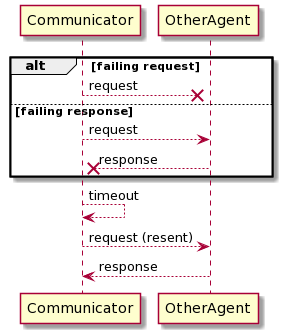
\includegraphics[width=.5\textwidth]{section/design/figure/agent/communicator_interaction.png}
    \caption{Esempio di gestione di failure di rete dell'agente \textit{Communicator}. Come precedentemente detto, per evitare una doppia 'risoluzione' della richiesta, \'e necessario che ogni messaggio abbia un identificativo che ne permetta il riconoscimento da parte (nell'esempio) di \textit{OtherAgent}.}
    \label{fig:communicator_sequence_diagram}
\end{figure}

\subsubsection{Admin}
Questo agente permette l'utilizzo delle funzionalit\'a di amministratore. A questo proposito, esso necessita di interagire con pi\'u entità del sistema, fra cui: \textit{WarehouseMapper} per lo storing e la rimozione degli elementi dal magazzino; \textit{CommandManager} per tutte le funzionalit\'a relative ai comandi. Inoltre, può potenzialmente dialogare con tutti gli agenti allo scopo di lanciare l'esecuzione dei comandi.\\
Un esempio relativo all'interazione necessaria all'esecuzione dei comandi \'e visibile in Figura \ref{fig:command_execution}

\subsubsection{User}
Come gi\'a detto il compito dell'user agent \'e relativo alla gestione degli ordini. A causa di ci\'o, la principale interazione di questo \'e con l'agente gestore degli ordini \textit{OrderManager} e con quello incaricato della gestione del magazzino, \textit{WarehouseMapper}, per la visualizzazione degli articoli disponibili.

\subsubsection{Collection Point Manager}
\subsubsection{Command Manager}
\subsubsection{Order Manager}
\subsubsection{Robot Picker}
\subsubsection{Warehouse Mapper}

\subsection{Considerazioni sul design scelto}
In questa sezione si ritiene interessante analizzare alcune scelte di design e le loro conseguenze. Nello specifico, si descriveranno alcuni approcci inizialmente intrapresi ma poi scartati o modificati nel corso del progetto. Inoltre, si descriveranno alcuni ragionamenti successivi allo sviluppo.

\subsubsection{Ontologia}
Il design dell'ontologia differiva inizialmente da quello descritto precedentemente nel capitolo, principalmente riguardo la struttura dei comandi. Questi erano definiti da un design molto pi\'u complicato comprendente `dipendenze' per l'esecuzione, `interfacce' e versioni (vedasi Figura \ref{fig:ontology-old-commands}).\\
I molti problemi legati a questa struttura (si pensi ad esempio alla risoluzione delle dipendenze cicliche) hanno poi portato alla scelta di una semplificazione della stessa, in quanto troppo complessa per il livello richiesto per l'esame.
\begin{figure}[!ht]\centering
    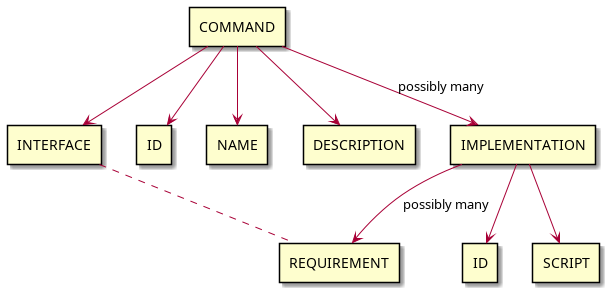
\includegraphics[width=\textwidth]{section/design/figure/ontology/ontology-old-commands.png}
    \caption{Design iniziale dei comandi. Ognuno consisteva di pi\'u implementazioni, le quali potevano dipendendere da alcune funzionalit\'a che l'agente doveva conoscere o reperire tramite una ricerca nel repository di piani.}
    \label{fig:ontology-old-commands}
\end{figure}
%
\subsubsection{Il modello di comunicazione}
Come gi\'a detto, uno scopo di questo progetto era l'apprendimento dell'utilizzo del modello di comunicazione a scambio di messaggi, in alternativa a quello basato su spazi di tuple visto a lezione. Questo modello si \'e invero rivelato molto flessibile nel suo utilizzo, tuttavia si \'e anche notato come per alcuni task sarebbe probabilmente stato pi\'u adatto un modello basato sullo spazio di tuple. In particolare, si \'e visto come tasks quali l'assegnamento di un oggetto da recuperare siano invero meglio rappresentati da un modello a spazio di tuple, dove gli agenti, una volta disponibili al compito, possano autonomamente accettare il task di recupero precedentemente pubblicato. Si nota infine come per altri task quali la sottomissione di un ordine, risulti invece pi\'u coerente il recapito diretto dei messaggi al singolo agente interessato.\\
In conclusione, non si considera la scelta fatta un errore, ma si ritiene comunque la considerazione sopra effettuata interessante ai fini della corretta comprensione del sistema e dei suoi punti deboli e di forza.
